\documentclass{cs-thesis}
\pagestyle{bachelorthesis}
\usepackage{listings,jlisting}
\usepackage[dvipdfmx]{graphicx}
\usepackage{appendix}
\usepackage{fancybox}
\usepackage{framed}
%\pagestyle{masterthesis}

\title{集合知と字句解析を用いた\\シンタックスハイライトの実現}
\author{趣味はマリンスポーツです}
\supervisor{0000 教授}
\studentnumber{00000000000-0}
\deadline{2012年2月13日}


\begin{document}


\titlepage

\abstract
 従来のシンタックスハイライトはプログラムの構造を見ず,正規表現による色付けを行うため,実際のソースコードと異なる色がつく問題がある.
 本論文では,ソースコードをクロールして得たトークンの出現確率,色付け対象のソースコードを字句解析して得たトークンの分類によって色付けを行う,シンタックスハイライトシステムを提案する.
 このシステムを利用することで,色付けの誤判定が少なくなり,結果が見やすく,さらに,ソースコードの構造が分かりやすくなることが期待できる.

\toc

 \section{はじめに}

 ソフトウェアの開発には,プログラミングが必須であり,多くのプログラミング言語が利用されている.
 また,一つのソフトウェアを作る際にも,複数のプログラミング言語を用いることが多い.
 例えば,Rubyでウェブアプリケーションを作る場合,メインのアプリケーションをRuby,データベースとのやりとりをSQL,表示部分をHTMLやテンプレート言語,クライアントサイドの動きをJavaScript,FlashはActionScript,のように,複数の言語を使うことが一般的である.
 ウェブアプリケーションのメインのプログラミング言語としても,Java,Ruby,Perl,PHP,Scalaなど,複数の選択肢がある.
 通常,プログラミングに用いるエディタは,プログラミングを支援する機能を持っている.
 構文のチェックや,プログラムの実行などをエディタから行えるようになっていたり,ソースコードが色分けされて見やすくなっていたりすると,プログラミングしやすくなる.
 しかしながら,構文のチェック方法やプログラムの実行方法は言語によって異なるので,エディタは言語別に支援機能を用意する必要があり,その手間は大きい.

 ここで,ソースコードを色分けして見やすくする機能をシンタックスハイライトという.
 ソースコードがシンタックスハイライトによって色分けされると,ソースコードを読みやすくなり,プログラムの構造が見やすくなり,エラーに気付きやすくなる.
 一般的なシンタックスハイライトは,プログラムの構造を見ず,正規表現のマッチングだけによって色付けをするため,シンタックスハイライトと実際のプログラムの構造が異なる場合がある.
 また,エディタ別,プログラミング言語別に独自の実装を行っているため,色に互換性がなく,エディタとプログラミング言語の組み合わせによって様々な色付けが行われる.

 本論文では,ソースコードをクロールし,集合知によって色を決定し,字句解析によってプログラムの構造を正しく理解した上でシンタックスハイライトを行うシステムを提案する.
 本システムを用いることで,ソースコードが正しく色付けされる従来のシンタックスハイライトでは得られなかった情報を見ることができ,プログラムの理解が進むといった利点が得られる.
 本システムはHTTPサーバーとして動作し,HTTP通信によって色を計算し,エディタは結果の表示のみを行うため,どのエディタを使っても等しい体験を得られるといった利点がある.

 本論文の構成は以下の通りである.
 2章でシンタックスハイライトについて説明する.
 3章で従来のシンタックスハイライト手法の問題点について述べ,本論文の提案するシンタックスハイライトシステムのアプローチと,システムの構成について述べる.
 4章で実行例を説明する.
 5章で考察を述べる.
 最後に6章でまとめを述べる.


 \clearpage
 \section{シンタックスハイライト}


  シンタックスハイライトとは,テキストエディタで,編集するソースコードが見やすくなるよう,色をつける機能である.
  予約語や変数名が色で区別できると,一目で見てプログラムの構造が分かりやすくなる.
  Eclipse,Emacs,Vim,Nano,TextMate,秀丸,TextMate,Geditといった一般的なプログラミングに用いられるテキストエディタにはシンタックスハイライトが実装されている.

  本節ではシンタックスハイライトについて説明し,一般的なテキストエディタにおけるシンタックスハイライト機能について説明する.

  
  \subsection{シンタックスハイライトの例}

  図\ref{emacs-without-syntax-highlight}と図\ref{emacs-with-syntax-highlight}にシンタックスハイライト前後でのソースコードの見た目の変化を示す.
  図\ref{emacs-without-syntax-highlight}において,ハイライト前は1色でただのテキストだったのが,図\ref{emacs-with-syntax-highlight}では,色分けされて,ソースコードが見やすくなっている.

    \begin{figure}[b]
   \centering
   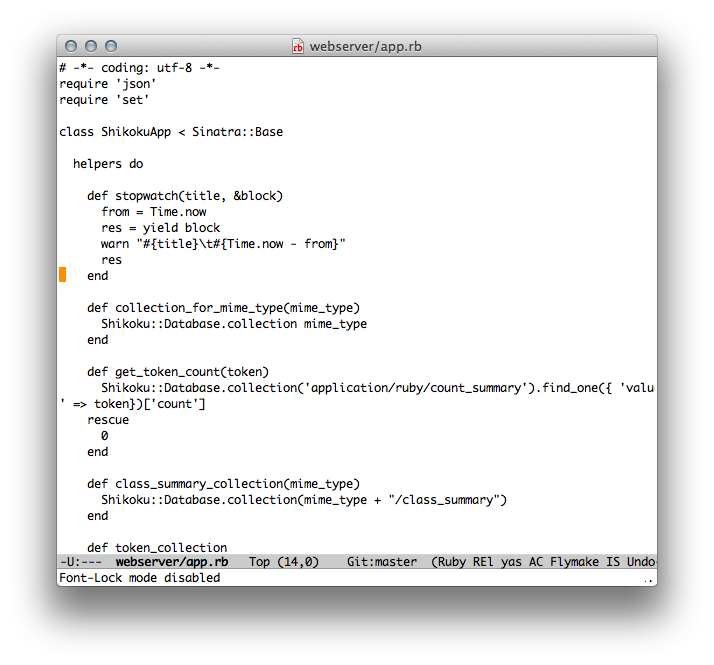
\includegraphics[scale=0.6]{emacs-without-syntax-highlight.png}
   \caption{シンタックスハイライト適用前のソースコード}
   \label{emacs-without-syntax-highlight}
  \end{figure}

  \begin{figure}[t]
   \centering
   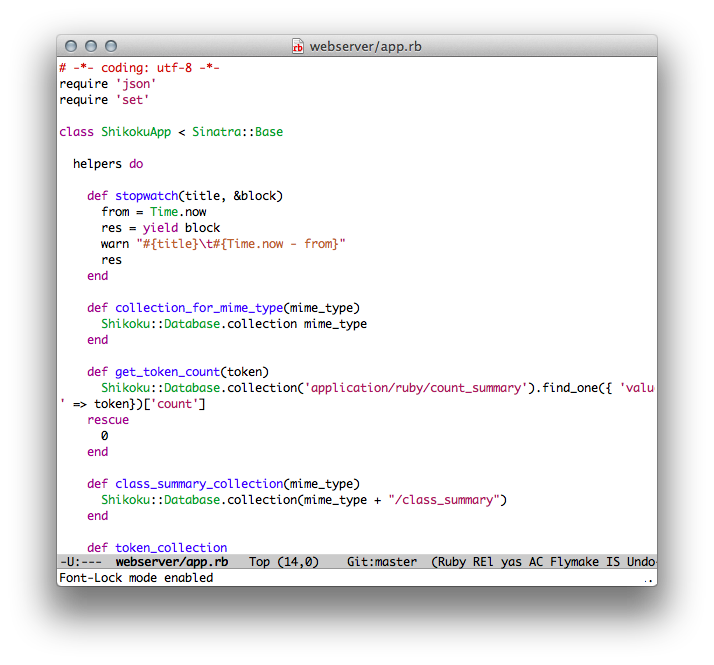
\includegraphics[scale=0.6]{emacs-with-syntax-highlight.png}
   \caption{シンタックスハイライト適用後のソースコード}
   \label{emacs-with-syntax-highlight}
  \end{figure}



  シンタックスハイライトは,色だけを変更し,フォントの種類やフォントサイズを変えないのが一般的である.
  Emacsのorg-mode\cite{bib:emacs-org}やyatex-mode\cite{bib:emacs-yatex}などのように,自然言語を編集する場合では,見出しを大きくするなど,フォントサイズを変えるものもある.

  同じキーワードについては同じ色を割り当てるのが一般的である.
  例えば,ifというキーワードが青い場合,他の場所のifも青いのが一般的である.
  ただし,ifというキーワードであっても,青くない場合もある.
  文字列リテラルの中のifという字は文字列リテラルの一部であってifというキーワードではないため,文字列リテラルの色がつく.

  シンタックスハイライトには見やすい色の組を選ぶ必要がある.
  背景が白で,薄い色をつかうと,コントラストが低くなり,ソースコードを読みにくい.
  また,意味の違う言葉に同じ色や似た色を割り当てると見間違いが生じる可能性がある.
  このため,なるべく,似た色は使わず,違いが分かる程度に色を分散させるのが一般的である.
  色は,予めシンタックスハイライトの設定で決められいて変更できない場合,あらかじめ用意された色の組み合わせから選べる場合,個別に設定できる場合がある.

  ハイライトのルールはハイライト対象の言語別に用意する必要がある.
  LispのシンタックスハイライトをCのプログラムに適用すると適切に色付けされない.
  Lispの予約語はCでは予約語ではないので,LispのシンタックスハイライトをCのプログラムに適用すると誤った色が付き,プログラムの構造が分かりにくくなる.

  シンタックスハイライトはエディタ別に実装されていて,エディタ間のシンタックスハイライトは振舞いは似ているが互換性がない.
  新しいエディタが生まれた際には,世に存在するプログラミング言語の数だけシンタックスハイライトをサポートする必要がある.
  ここでは,テキストエディタ,nano,Vim,Emacsを取り上げ,シンタックスハイライトの具体的な設定を示す.

  \clearpage
  \subsubsection{nanoにおけるシンタックスハイライト}
  テキストエディタのnano\cite{bib:nano}では,.nanorcという設定ファイルを編集することで,エディタの振舞いを変更できる.
  nano本体の機能として,シンタックスハイライト機能がある.

  Pythonのシンタックスハイライトを有効にするには,nanorcから,以下のように,python.nanorcを読み込む.

  \begin{framed}
\begin{verbatim}
## Python
include "/usr/share/nano/python.nanorc"

\end{verbatim}
\end{framed}

  python.nanorcにはPython用のシンタックスハイライトの設定が書かれている.
  python.nanorcの内容を示す.

  \begin{framed}
\begin{verbatim}
## Here is an example for Python.
##
syntax "python" "\.py$"
header "^#!.*/python[-0-9._]*"
icolor brightblue "def [0-9A-Z_]+"
color brightcyan "\<(and|as|assert|break|class|continue|def|del|elif
        |else|except|exec|finally|for|from|global|if|import|in|is
        |lambda|not|or|pass|print|raise|return|try|while|with|yield)\>"
color brightgreen "['][^']*[^\\][']" "[']{3}.*[^\\][']{3}"
color brightgreen "["][^"]*[^\\]["]" "["]{3}.*[^\\]["]{3}"
color brightgreen start=""""[^"]" end=""""" start="'''[^']" end="'''"
color brightred "#.*$"

\end{verbatim}
 \end{framed}

  以下のような設定が書かれている.

  \begin{itemize}
   \item ファイル名が.pyで終わるときにPythonのシンタックスハイライトを有効にする.
   \item Shebangにpythonが含まれるときPythonのシンタックスハイライトを有効にする.
   \item def [0-9A-Z\_]+ にマッチする部分は明い青色にする.
   \item and または as または assert または break など,予約語にマッチするときは明るい青緑にする.
  \end{itemize}

  色をつける箇所は正規表現で書かれている.

  nanoのシンタックスハイライトでは,ハイライトの設定で色まで決められていて,ユーザーは色を変更することができない.上の例では,Pythonの予約語は常に明るい青緑で表示される.

  \subsubsection{Vimにおけるシンタックスハイライト}
  Vim\cite{bib:vim}では.vimrcというファイルに以下の設定を書き,syntax機能を有効にすることで,シンタックスハイライトを有効にできる.
  syntaxをenableにすると自動的に各言語用の設定が読み込まれる.

\begin{framed}
\begin{verbatim}
 :syntax enable
\end{verbatim}
\end{framed}

  nanoでは,シンタックスハイライトのルールに色まで決めていたが,vimでは,シンタックスハイライトのルールでは,トークンのクラスまでを決めている.
  トークンのクラスだけを正規表現で切り出し,そのクラスに対応する色は別の設定で決める.
  これによって,各言語用に正しいシンタックスハイライトの設定が用意されていれば,編集する言語によらず,statementは緑,といったように,一貫性が保たれる.
  また,Vimスクリプトというスクリプト言語を実行することができ,プログラムによって色付けできる.

  VimではVimScriptというスクリプト言語で設定を書くことができ,シンタックスハイライトの振舞いを設定することができる.
  以下の例では,python\_highlight\_allという変数をtrueにしているときには,ハイライトするルールを増やす,ということが書かれている.

  \begin{framed}
\begin{verbatim}
if exists("python_highlight_all")
  let python_highlight_numbers = 1
  let python_highlight_builtins = 1
  let python_highlight_exceptions = 1
  let python_highlight_space_errors = 1
endif

if exists("python_highlight_numbers")
  " numbers (including longs and complex)
  syn match   pythonNumber	"\<0x\x\+[Ll]\=\>"
  syn match   pythonNumber	"\<\d\+[LljJ]\=\>"
  syn match   pythonNumber	"\.\d\+\([eE][+-]\=\d\+\)\=[jJ]\=\>"
  syn match   pythonNumber	"\<\d\+\.\([eE][+-]\=\d\+\)\=[jJ]\=\>"
  syn match   pythonNumber	"\<\d\+\.\d\+\([eE][+-]\=\d\+\)\=[jJ]\=\>"
endif

\end{verbatim}
 \end{framed}

  どのクラスがどの色か,という対応は,カラースキームを選ぶことで決められる.
  下にカラースキームの定義の例を示す.Statementというクラスは,VimがGUIで起動していて,フルカラー表示できるときは文字色は\#dfdf6f,これはRGBで,R = 223,G = 223,B = 111,という意味である,それ以外で,ターミナル内に起動している場合は,yellowという色が割り当てられる.
  カラースキームには,文字のクラスごとに,文字色,背景色,文字の装飾(太字かどうか),が定義されている.
  nanoでは最初に決められた通りに色付けされるだけだったのが,Vimでは,ユーザーが色や振舞いを変える仕組みが用意されている.

  \begin{framed}
\begin{verbatim}
hi Identifier   guifg=#dfdf6f       guibg=NONE          gui=NONE
            \   ctermfg=yellow      ctermbg=NONE        cterm=NONE

hi Statement    guifg=#6fef7f       guibg=NONE          gui=bold
            \   ctermfg=green       ctermbg=NONE        cterm=bold

hi PreProc      guifg=#afafaf       guibg=NONE          gui=NONE
            \   ctermfg=darkgreen   ctermbg=NONE        cterm=NONE

hi Type         guifg=#9f9fef       guibg=NONE          gui=bold
            \   ctermfg=lightblue   ctermbg=NONE        cterm=bold

\end{verbatim}
 \end{framed}

  \subsubsection{Emacsのシンタックスハイライト}
  Emacs\cite{bib:emacs}では,オーバーレイという仕組みがあり,テキストにオーバーレイを設定することで,色やフォントなどの見た目を変更できる.
  fontlock-modeというシンタックスハイライトをするためのメジャーモードを使うと,簡単にシンタックスハイライトを実装できる\cite{bib:emacs-oreilly}.
  各言語のfontlock-mode用の設定を書くと色付けできる.
  また,Vimと同様に,font-lock-variable-name-face のように,変数名の色を決められる.

  fontlock-modeは,他のシンタックスハイライト機能と同様に,キーワードや正規表現のリストをもとに色付けしているが,自力でオーバーレイを組み立てることで,独自にシンタックスハイライトを実装することができる.

  js2-modeは,Emacs Lispで書かれたJavaScriptパーサーを持っており,Emacs上でJavaScriptのソースコードをコンパイルして色付けしている.
  しかし,Emacs LispでJavaScriptをパーサーを書くのは,正規表現を用意するだけに比べると手間が大きい.
  nanoのPythonの設定が10行程度であるのに対し,Emacsのjs2-modeは1万1000行もある.

  \subsection{字句解析}
  多くのプログラミング言語では,その最小構成として字句(トークン)を定義している.
  このため,シンタックスハイライトを実現する際に,編集中のプログラムから字句を取り出せると都合が良い.
  一般的には,この作業を字句解析と言い,これを実装したものが字句解析器である\cite{bib:compiler}.

  字句解析器はコンパイラの一部として組込まれていることが多いが,独立して呼び出せるものがある.
  独立して呼び出し,字句解析できるモジュールとして,RubyのRipper,Pythonのtokenize,PerlのPPIなどがある.
  ただし,これらのモジュールは,スクリプト言語のインタプリタが実行前に呼び出しているものではなく,スクリプト言語の仕様に沿って実装し直されたものである.

  順に,これらの字句解析モジュールの使い方や,得られる情報について説明する.

  \subsubsection{Rubyの字句解析}

  以下にRipperを用いてRubyのソースコードを字句解析する例を示す.
  Ripperを呼び出すプログラムは以下である.

\begin{framed}
\begin{verbatim}
require 'ripper'
require 'pp'

pp Ripper.lex(ARGF.read)
\end{verbatim}
\end{framed}

以下のプログラムを字句解析する.

\begin{framed}
\begin{verbatim}
a = (3.5 - 1.2) * 4
puts a
\end{verbatim}
\end{framed}

すると,以下の結果が得られる.

\begin{framed}
\begin{verbatim}
[[[1, 0], :on_ident, "a"],
 [[1, 1], :on_sp, " "],
 [[1, 2], :on_op, "="],
 [[1, 3], :on_sp, " "],
 [[1, 4], :on_lparen, "("],
 [[1, 5], :on_float, "3.5"],
 [[1, 8], :on_sp, " "],
 [[1, 9], :on_op, "-"],
 [[1, 10], :on_sp, " "],
 [[1, 11], :on_float, "1.2"],
 [[1, 14], :on_rparen, ")"],
 [[1, 15], :on_sp, " "],
 [[1, 16], :on_op, "*"],
 [[1, 17], :on_sp, " "],
 [[1, 18], :on_int, "4"],
 [[1, 19], :on_nl, "\n"],
 [[2, 0], :on_ident, "puts"],
 [[2, 4], :on_sp, " "],
 [[2, 5], :on_ident, "a"],
 [[2, 6], :on_nl, "\n"]]
\end{verbatim}
\end{framed}

出力結果は,3要素のタプルのリストになっていて,内容は,トークンの出現位置の(行,桁),トークンの種類,トークンの文字列,である.
空白や改行も出力されるので,連結すればもとのソースコードを復元することができる.

  \subsubsection{Pythonの字句解析}
  Pythonのtokenizeの使用例を示す.

tokenizeを呼び出すプログラムは以下である.
\begin{framed}
\begin{verbatim}
#!/usr/bin/env python
import sys
import tokenize

generator =  tokenize.generate_tokens(sys.stdin.readline)

for token_class, token_value, start, end, line in generator:
    print [token_class, token_value, start, end, line]
\end{verbatim}
\end{framed}

以下のプログラムを字句解析する.
\begin{framed}
\begin{verbatim}
a = (3.5 - 1.2) * 4
print a
\end{verbatim}
\end{framed}

すると以下が出力される.
\begin{framed}
\begin{verbatim}
[1, 'a', (1, 0), (1, 1), 'a = (3.5 - 1.2) * 4\n']
[51, '=', (1, 2), (1, 3), 'a = (3.5 - 1.2) * 4\n']
[51, '(', (1, 4), (1, 5), 'a = (3.5 - 1.2) * 4\n']
[2, '3.5', (1, 5), (1, 8), 'a = (3.5 - 1.2) * 4\n']
[51, '-', (1, 9), (1, 10), 'a = (3.5 - 1.2) * 4\n']
[2, '1.2', (1, 11), (1, 14), 'a = (3.5 - 1.2) * 4\n']
[51, ')', (1, 14), (1, 15), 'a = (3.5 - 1.2) * 4\n']
[51, '*', (1, 16), (1, 17), 'a = (3.5 - 1.2) * 4\n']
[2, '4', (1, 18), (1, 19), 'a = (3.5 - 1.2) * 4\n']
[4, '\n', (1, 19), (1, 20), 'a = (3.5 - 1.2) * 4\n']
[1, 'print', (2, 0), (2, 5), 'print a\n']
[1, 'a', (2, 6), (2, 7), 'print a\n']
[4, '\n', (2, 7), (2, 8), 'print a\n']
[0, '', (3, 0), (3, 0), '']
\end{verbatim}
\end{framed}

tokenizeの出力結果は5要素のタプルのジェネレータで,トークンの型,トークンの文字列,トークンの開始位置(行,列),トークンの終了位置(行,列),トークンの見つかった行の文字列,である.
開始位置と終了位置は文字単位である.
空白はトークンとして現れないので,もとのソースコードを復元するには,開始位置と見比べて空白を挿入する必要がある.

トークンの型は数値として返される.上の例では,'a'の型は1と出力されている.そのままでは見ても意味が分からないが,tokenモジュールを使うと,人間が見て理解できる形式に変換できる.
tokenモジュールは,token.tok\_nameという,トークンの型がキーでトークンの型名が値のハッシュを持っている.
以下のプログラムでは,トークンの型が文字列として出力される.

\begin{framed}
\begin{verbatim}
#!/usr/bin/env python
import sys
import tokenize
import token

generator =  tokenize.generate_tokens(sys.stdin.readline)

for token_class, token_value, start, end, line in generator:
    print [token.tok_name[token_class], token_value, start, end, line]
\end{verbatim}
\end{framed}

\begin{framed}
\begin{verbatim}
['NAME', 'a', (1, 0), (1, 1), 'a = (3.5 - 1.2) * 4\n']
['OP', '=', (1, 2), (1, 3), 'a = (3.5 - 1.2) * 4\n']
['OP', '(', (1, 4), (1, 5), 'a = (3.5 - 1.2) * 4\n']
['NUMBER', '3.5', (1, 5), (1, 8), 'a = (3.5 - 1.2) * 4\n']
['OP', '-', (1, 9), (1, 10), 'a = (3.5 - 1.2) * 4\n']
['NUMBER', '1.2', (1, 11), (1, 14), 'a = (3.5 - 1.2) * 4\n']
['OP', ')', (1, 14), (1, 15), 'a = (3.5 - 1.2) * 4\n']
['OP', '*', (1, 16), (1, 17), 'a = (3.5 - 1.2) * 4\n']
['NUMBER', '4', (1, 18), (1, 19), 'a = (3.5 - 1.2) * 4\n']
['NEWLINE', '\n', (1, 19), (1, 20), 'a = (3.5 - 1.2) * 4\n']
['NAME', 'print', (2, 0), (2, 5), 'print a\n']
['NAME', 'a', (2, 6), (2, 7), 'print a\n']
['NEWLINE', '\n', (2, 7), (2, 8), 'print a\n']
['ENDMARKER', '', (3, 0), (3, 0), '']
\end{verbatim}
\end{framed}

上と比べると,'a'の型名が'NAME'と表示され,分かりやすくなった.

  \subsubsection{Perlの字句解析}
PerlのPPIは字句解析のみを行う機能はなく,呼び出すと構文解析まで行う.
構文木を順番に見て,tokenなら表示する,という方法で,トークンのリストを得られる.
トークンはPPI::Tokenクラスの子クラスで,トークンの種類に対応したクラスのインスタンスなので,ref関数を用いて,トークンのクラスを取得すると,トークンの種類を得られる.
空白や改行もトークンとして出力されるので,トークンの文字列を連結すればもとのソースコードを復元できる.

以下はPPIを呼び出して構文木を作り,トークンの列を出力するプログラムである.

\begin{framed}
\begin{verbatim}
use strict;
use warnings;
use Perl6::Say;
use PPI;

say join "\n", map {
    join ", ",  ref $_, "'" . $_->content . "'";
} @{PPI::Document->new(\ join ('', <STDIN>, "\n"))->find(q{PPI::Token})};
\end{verbatim}
\end{framed}

以下のプログラムを字句解析する.

\begin{framed}
\begin{verbatim}
$a = (3.5 - 1.2) * 4;
print $a;
\end{verbatim}
\end{framed}

以下の結果が出力される.

\begin{framed}
\begin{verbatim}
PPI::Token::Symbol, '$a'
PPI::Token::Whitespace, ' '
PPI::Token::Operator, '='
PPI::Token::Whitespace, ' '
PPI::Token::Structure, '('
PPI::Token::Number::Float, '3.5'
PPI::Token::Whitespace, ' '
PPI::Token::Operator, '-'
PPI::Token::Whitespace, ' '
PPI::Token::Number::Float, '1.2'
PPI::Token::Structure, ')'
PPI::Token::Whitespace, ' '
PPI::Token::Operator, '*'
PPI::Token::Whitespace, ' '
PPI::Token::Number, '4'
PPI::Token::Structure, ';'
PPI::Token::Whitespace, '\n'
PPI::Token::Word, 'print'
PPI::Token::Whitespace, ' '
PPI::Token::Symbol, '$a'
PPI::Token::Structure, ';'
PPI::Token::Whitespace, '\n'
PPI::Token::Whitespace, '\n'
\end{verbatim}
\end{framed}

  \clearpage
 \section{シンタックスハイライトシシテム}
 2章では,一般的なシンタックスハイライトについて説明した.
 本章では,シンタックスハイライトの問題について述べ,これらを解決するシンタックスハイライトシステムを提案する.

  \subsection{シンタックスハイライトの問題点}
  2章で述べたシンタックスハイライトには以下の問題がある.
  \begin{itemize}
   \item ルールが間違っていて,正しく色付けできない場合があること
   \item ルールはエディタ間で共通化されていないこと
   \item 識別子であっても,誤っていることが示されないこと
  \end{itemize}

  順に説明する.

  \subsubsection{ルールが間違っている}
  プログラムを正しく理解して色をつけるにはプログラムの構造を正しく認識する必要がある.
  このため,字句解析や構文解析が必要であるが,一般的なシンタックスハイライトは,正規表現などで色をつけている.
  よって,誤認識されて,実行時とは異なる構造が示されることがある.

  図\ref{emacs-class-aaa}は,EmacsのRubyモードにおける誤認識の例である.
  class\_aaaという変数名の,classの部分に,クラスを宣言するときに利用するclassキーワードの色が誤って割り当てられている.


  \begin{figure}[htbp]
   \centering
   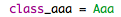
\includegraphics[scale=0.8]{emacs-class-aaa.png}
   \caption{誤認識の例}
   \label{emacs-class-aaa}
  \end{figure}



  図\ref{emacs-divide}はEmacsのCoffeeScriptモードの誤認識の例である.2回の割り算が正規表現リテラルの色だと誤認識されて色付けされている.


  \begin{figure}[htbp]
   \centering
   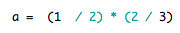
\includegraphics[scale=0.8]{emacs-divide.png}
   \caption{誤認識の例}
   \label{emacs-divide}
  \end{figure}

  色付けの正規表現のルールを間違うと正しく色付けされない.
  誤った色付けに応じてプログラムの構造を誤って捉えると,ソフトウェアを誤って理解してしまうことがある.
  正しく色付けすることはシンタックスハイライトの課題である.

  また,誤認識ではないが,プログラムに誤りがあるとき,見にくい色がつくことがある.
  文の先頭に誤ってクオートが1つだけ入っているとき,クオート以降のプログラム全体がストリングリテラルだと認識されて,プログラム全体が変な色になる.
  図\ref{emacs-right-delimiter}は正しくコンパイルできるソースコードであり,正しく色付けされている.
  図\ref{emacs-wrong-delimiter}は誤ったソースコードで,defの前に誤って''(ダブルクオート)が入っていて,retrieveというストリングまでがストリングリテラルだという扱いになっている.
  プログラムが正しくないために,どのような色を付けるのが正しいかはといった指標はないが,シンタックスハイライトはプログラムを色分けしてプログラムの構造を示すためのものなので,プログラム全体が単一の色で塗られているのは見にくい.


  \begin{figure}[b]
   \centering
   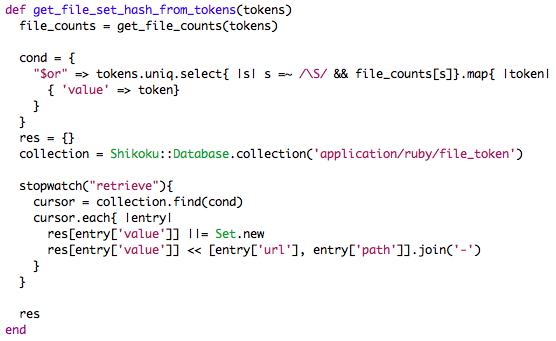
\includegraphics[scale=0.7]{emacs-right-delimiter.png}
   \caption{正しく色付けされたソースコード}
   \label{emacs-right-delimiter}
  \end{figure}

  \begin{figure}[t]
   \centering
   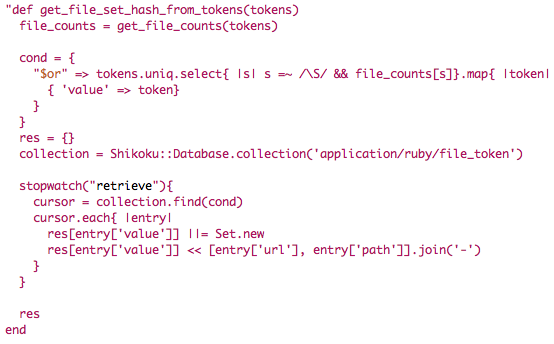
\includegraphics[scale=0.7]{emacs-wrong-delimiter.png}
   \caption{誤って色付けされたソースコード}
   \label{emacs-wrong-delimiter}
  \end{figure}

  このように,既存の手法では,正しいソースコードでも正しく色付けされない場合や,正しくないソースコードの場合に見にくい色付けがされる場合がある.
  これらは全て,正規表現で色をつけているのが原因である.正規表現のルールが正しくないために,1つのトークンが2つの色で塗られたり,3つのトークンがまとめて1色で塗られたり,プログラム全体が1つの色で塗られたりする.

  \subsubsection{互換性がない}
  エディタや言語別に様々なシンタックスハイライトの実装がある.
  このため,それぞれに互換性がなく,個別にメンテナンスしていく必要がある,という問題がある.
  たとえば,処理系のバージョンが上がり,予約語が増えたとき,各エディタのその言語のシンタックスハイライトのルールを修正する必要がある.
  JavaScript1.7にはyieldという予約語が増えたので,各エディタのシンタックスハイライトプログラムを修正してyieldに予約語の色をつける必要がある.

  予約語のリストはエディタを問わず一定なので,共有できてもよいはずである.
  エディタ間でシンタックスハイライトのルールを共有することができれば,世の中で1つだけルールを保守すればよいということになり,シンタックスハイライトプログラムの保守が楽になる.

  \subsubsection{誤っていることが示されない}
  シンタックスハイライトによって,識別子であることは分かるが,その識別子が世の中でどの程度使われているものなのか,ということは分からない.
  そのため,libraryという識別子を誤ってlibralyなどと書いていても,プログラムとして動作すれば,綴りの誤りに気付かない.
  libralyのような綴り間違いの場合は,英語の辞書を用いることで間違いを検出できる.
  しかし,BufferedReaderと書くべきところを,BufferReaderと書くなど,英語として意味の通じるような間違いの場合は,辞書を使っても判断できない.
  また,組織内でのみ使われる単語は,一般的な辞書には載っていない.

  スペル間違いの識別子を見つけるという他に,識別子がどのくらいの頻度で使われるものか分かると,プログラムを書いたり読んだりする際に役に立つと思われる.
  プログラムを書いたときに,よく使われるものと思って書いた識別子の出現頻度が低いと,何か思い違いをしている可能性がある.
  たとえば,Rubyでライブラリをロードするには,requireというメソッドと,loadというメソッドがあるが,一般的に,requireはloadより多く使われる.
  requireでロードされたときにはライブラリは一度だけロードされるのに対し,loadは既にロード済みのライブラリでも再度読み込むため,requireのかわりにloadを使うとパフォーマンス上問題がある.
  単にライブラリをロードしようとしてloadと書くと,loadの出現確率は低いため,何か変だということに気付くことができる.

  識別子が一般的かどうかは,辞書では判定できない.
  世の中のソースコードを集めて,解析して,出現確率を調べることで,一般的かどうかが分かる.

 \subsection{アプローチ}
 本論文は,正規表現を使わず,字句解析を用い,エディタによらず動作し,識別子のもっともらしさも同時に示す,シンタックスハイライトを行うシステムを提案する.

 本システムは,正規表現によるルールを用いず,色付け対象のソースコードの字句解析を行い,その結果をもとに,色付けする.
 これにより,ルールが誤っていて,正しい構造が示されないという問題が解消されることが期待できる.

 本システムは,サーバークライアント型モデルを採用し,シンタックスハイライトを行うアプリケーションをシンタックスハイライトサーバーとして動作させ,エディタにはサーバーと通信して結果を表示する処理のみを実装する.
 これにより,どのようなエディタを使っても,一定の色付け結果を得ることを目指す.

 本システムは,トークンのクラスを示すだけでなく,クロールされたデータをもとに,統計的に,トークンが世の中でどのくらい利用されているかも同時に示す.
 これにより,綴り間違いや,一般的でない名前をつけてしまう,という問題が解消されることを目指す.

  \subsection{システムの概要}
  本システムの構成を図\ref{system}に示す.
  本システムはHTTPサーバとHTTPクライアントであるテキストエディタから成る.
  以下,HTTPサーバーとソースコードエディタについて説明する.

    \begin{figure}[htbp]
   \centering
   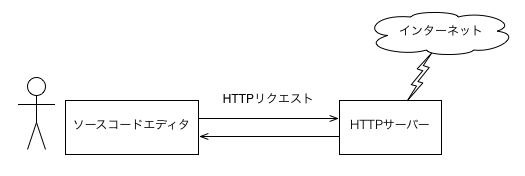
\includegraphics[scale=0.8]{system.png}
   \caption{本システムの構成}
   \label{system}
  \end{figure}

  \subsubsection{HTTPサーバー}
    本システムは,HTTPサーバーとして動作し,HTTP POSTリクエストとしてソースコードを受け取り,HTTPレスポンスとしてトークンごとの色情報を返すHTTPサーバーとして動作する.

  リクエストのパラメータは以下である.

  \begin{itemize}
   \item body: ソースコードの本文
   \item mime\_type: ソースコードの言語に対応したmime type
  \end{itemize}

  レスポンスのパラメータは以下である.

  \begin{itemize}
   \item is\_valid: 入力されたソースコードの字句解析に成功したかどうか
   \item tokens: 入力されたソースコードのトークンを示すオブジェクトの配列をJSON形式でシリアライズしたもの
  \end{itemize}

  オブジェクトは以下のキーを持つ.
  \begin{itemize}
   \item value: トークンの文字列
   \item token\_class: トークンのクラス
   \item color: トークンの色
   \item count: データベースに記録されているトークンの出現回数
   \item rate:  データベースに記録されているトークンの出現頻度
  \end{itemize}

  トークンの色はhsl(H, S, L) という形式の文字列で表現される.

  リクエストが正しく,正しいレスポンスを返せるときは,レスポンスにStatus Codeとして200 (Success) を返す.
  bodyやmime\_typeが入力されないときや,入力されたmime\_typeに対応する字句解析モジュールがシステムにない場合は,Status Codeとして400 (Bad Request)を返す.
  文字コードはUTF-8を対象としている.

  本システムはRubyで書かれているが,HTTPリクエストを経由して入力を受け付けることで,HTTP通信できるプログラミング言語から利用することができる.
  Emacsから利用するときはEmacs Lispを用いて通信し,Vimから利用するときはVimスクリプトを用いて通信することができる.
  本システムのレスポンスはJSON形式で返されるが,Emacsではjson.elというライブラリを使うとJSONをパースすることができる.Vimでは,外部プロセスとして何らかのスクリプト言語を呼び出し,スクリプト言語が,Vimで扱える形式にデータ構造を変換すると良いと思われる.

  \subsubsection{ソースコードエディタ}
  本システムはウェブブラウザ上で動作するソースコードエディタを持っている.

  本システムは,本来はEmacs等のソースコードエディタと協調して動くことを想定して作られている.
  しかし,実際にEmacs等のプラグインを実装する時間がなかったため,プロトタイプとして,簡単に実装できる,ウェブブラウザ上で動作するソースコードエディタを実装した.

  言語を選び,テキストエリアにソースコードを入力すると,JavaScriptで本システムと通信し,色付け結果をHTMLとして提示する.
  本来のシンタックスハイライトはユーザーが入力した文字に色をつけるものであるが,ウェブブラウザ上では,ユーザーが入力した文字の色を変えることができなかったため,色付け済の文字を下に並べて表示している.

  \subsection{システムの処理の流れ}
  本システムの処理の流れを図\ref{flow}に示す.
  四角は処理を,二重線はデータを表す.
  本システムは,前段階として,インターネット上からソースコードをクロールして集め,字句解析し,その結果をデータベースに保存しておく.
  本システムは,ソースコードを色付け対象のソースコードをHTTP POSTメソッドを用いて受信し,字句解析し,トークンのクラスと,そのトークンの出現確率によって色を決め,JSON形式でエディタに返す.JSONはJavaScript Object Notationで,JavaScriptにおけるオブジェクトの表記法をもとにしたフォーマットである.

  テキストエディタは本システムのHTTPサーバーにHTTPリクエストを送信し,受信した情報によってソースコードの色付けを行う.
  実際のテキストエディタに組込むかわりに,ウェブブラウザ上で動作する簡易的なソースコードエディタを提供する.

  以下,それぞれの処理について説明する.

  \begin{figure}[htbp]
   \centering
   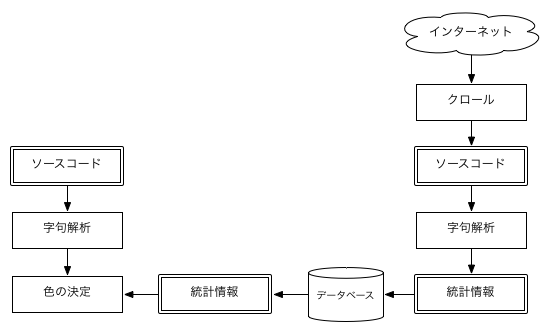
\includegraphics[scale=0.8]{flow.png}
   \caption{本システムの処理の流れ}
   \label{flow}
  \end{figure}

  \clearpage
  \subsubsection{クロール}
  本システムはソースコードをGitHubからクロールしてデータベースに保持する.

  GitHubはGitのホスティングサービスである.
  Gitは分散型のバージョン管理システムである.
  GitHubはオープンソース開発で活発に使われていて,RubyのウェブアプリケーションフレームワークであるRuby on Railsや,Macのパッケージ管理ツールであるHomebrewなど,多くの有名なプロジェクトがGitHub上で開発されている.

  GitHubには,ブックマーク機能があり,注目しているプロジェクトをブックマークに登録することができ,プロジェクトを見たり検索したりする際に,ブックマークに多く登録された順にプロジェクトを見ることができる.
  GitHubには,リポジトリに登録されたソースコードの言語を判定する機能があり,プロジェクトで使われている主な言語によってプロジェクトを検索することができる.

  本システムのクローラは,起動時に言語を指定すると,指定された言語のプロジェクトを検索し,ブックマークに多く登録された順にソースコードをダウンロードする.
  ユーザーが終了するまで動き続ける.

  ダウンロードしたソースコードは,本システムに対応した字句解析器がある場合は,字句解析され,データベースに保存される.

  データベースに登録されるものは以下である.
  データベースは,ソースコードの言語別にテーブルが分けられている.

  ファイル単位で,fileテーブルに,以下のレコードを作る.

\begin{itemize}
 \item url: ファイルが含まれるリポジトリのURL
 \item path: リポジトリ内のファイルのパス
 \item mtime: ファイルの最新更新日時
 \item mime\_type: ファイルの内容,例えば,Rubyのソースコードなら,application/ruby
\end{itemize}

  また,トークン単位で,tokenテーブルに,以下のレコードを作る.
  ただし,同じ文字列のトークンのレコードがデータベースに既にある場合は,新しくレコードを作らず,出現回数を増やす.
  ただし,空白は色をつけられないので,空白のみから成るトークンはデータベースに保存しない.
  ただし,1ファイルにつき,トークンのカウントを増やせるのは,1回とする.
  あるファイルに,requireというキーワードが複数出現しても,カウントは1だけ増やす.
  countは,そのトークンがいくつのファイルで出現しているか,を示す.
  token\_classは,出現するたびにカウントしていく.

  \begin{itemize}
   \item value: トークンの文字列
   \item count: トークンの出現回数
   \item token\_class: トークンの字句解析上のクラスのハッシュ,キーはトークンのクラスで,値は出現回数
  \end{itemize}

  ソースコードの言語の判定には,shared-mime-infoという,ファイルの拡張子と内容からファイルの内容を判定するライブラリを用いている.
  mime infoは,HTTP通信におけるContent-Typeを判定するためのモジュールである.
  ウェブブラウザは,HTTPレスポンスのContent-Typeヘッダによって,表示方法を変更している.
  たとえば,text/htmlというContent Typeが送られてきたときは,受信した本文をHTMLとして表示するが,image/jpegというContent Typeを受信したときは,受信内容をJpeg形式の画像として表示する.
  shared-mime-infoは,ウェブサーバーの静的ファイル配信に用いられるライブラリで,あるディレクトリ以下にあるファイルを配信したい,といった用途のときに,a.jpgのようなファイル名と,そのファイルの内容から,適切なContent-Typeを得るために使われている.
  本システムでは,クロールして集めたソースコードの言語を判定して,適切な字句解析器に渡すために用いている.
  ファイル名だけで判定できない理由としては,拡張子が与えられていないときに,ソースコードが何であるか判定できないため,shared-mime-infoを用いた.
  また,拡張子がjavaであっても,内容がJpeg画像の場合は,Javaのソースコードとして扱うことはできないため,ファイルの内容を見て判定することが必要だと考えた.

  データベースとして,MongoDBを用いた.
  MongoDBはスキーマレスなデータベースで,JSONを拡張した形式でオブジェクトを格納できる.そのため,ハッシュのようなデータ構造をデータベースに保存できる.
  スキーマレスなため,実装時のプロトタイピングに向いていると考え,MongoDBを用いることにした.

  クロールされたソースコードはファイルシステム上に保存される.
  ソースコードは,単なるダウンロードではなく,Gitリポジトリのクローンという形でダウンロードする.
  そのため,クローラは,最初は全ファイルをダウンロードするが,次回以降ダウンロードする場合は,前回ダウンロードしたバージョンからの差分だけをダウンロードすることで,最新のバージョンのリポジトリを入手することができる.
  初回はGit Cloneというコマンドでクローンし,次回以降は,Git Pullというコマンドで最新バージョンをチェックアウトする.
  再ダウンロードした場合は,データベースから,前のバージョンのレコードを削除し,新しいバージョンのレコードを入れることで,データベースを最新化することができる.


  \subsubsection{字句解析}

  本システムでは,二カ所で字句解析を行う.
  一箇所目は,クロールしたソースコードをデータベースに保存するときである.
  二箇所目は,クライアントが送信したソースコードの色情報を計算するときである.

  本システムの字句解析モジュールは,RubyとPythonとPerlに対応している.
  内部的には,RubyのRipper,Pythonのtokenize,PerlのPPIを呼び出し,結果を配列で受け取っているので,新しい言語用の字句解析モジュールを書けば,対応言語を増やすことができる.

  字句解析モジュールは,入力としてソースコードを受け取り,出力として,トークン文字列とクラスの配列,字句解析に成功したかどうかを返す.
  クラスの内容は字句解析モジュールに依存している.たとえば,Rubyの字句解析モジュールはon\_identのようなクラスを返し,Pythonの字句解析モジュールはNAMEのようなクラスを返す.
  クラス名は,クラス名の出現確率に応じた色を決定するために使われる.

  クロールしたソースコードをデータベースに保存するときに字句解析に失敗した場合は,そのソースコードをデータベースに保存しない.
  誤ったソースコードをデータベースに登録すると,情報の質が悪くなるためである.

  クライアントから送信されたソースコードの字句解析に失敗した場合は,正規表現で,空白と単語境界によって適当にトークンを切り分ける.
  切り分けるだけではトークンのクラスが分からないため,以下の方法でデータベースからトークンのクラスを推測する.
  \begin{itemize}
   \item tokenテーブルから,トークンの文字列が一致するレコードを取得する
   \item レコードが存在しないとき,クラスは不明とする
   \item レコードが存在したとき,token\_classフィールドのうち,出現回数が一番大きいものをトークンのクラスとして採用する
  \end{itemize}

  トークンのクラスはトークンの文字列から一意に決定できない.字句解析して,前後のトークンとの関係を見なければならない.
  字句解析に失敗しているので,字句解析によって決定することはできないので,確率の一番大きいものをクラスとする.
  たとえば,/という文字は,Rubyにおいては,以下の4つのクラスが考えられる.
  \begin{itemize}
   \item 割り算のオペレータ
   \item 正規表現リテラルの開始
   \item 正規表現リテラルの終了
   \item ``/''という文字列リテラルの内容
  \end{itemize}

  本システムでは,トークンのクラスによって色を決めているので,正しいクラスを推測しなければ,正しい色をつけることはできない.
  しかし,字句解析に失敗するソースコードに完全に正しいクラスを割り当てることは不可能である.
  正しいクラスを割り当てできるとすると,字句解析に成功するということになってしまう.

  \subsubsection{色の決定}
  本システムは,トークンの文字列とクラスの配列から,トークンごとに色を決定する.
  色は,文字色だけを決め,背景色や文字サイズ,フォントの種類などは変更しない.
  以下のルールによって色を決める.
  \begin{itemize}
   \item よく出現する文字列は暗い
   \item よく出現するクラスは青い
  \end{itemize}
  したがって,一般的なソースコードは,青く,暗くなる.
  一般的でないソースコードは,赤く,薄くなる.

  本システムの色は二次元情報である.
  本システムの利用者はソースコードの色の二次元的な情報と,ソースコード自体の意味を同時に見て情報を得ることができる.

  本システムのソースコードは,よく出現する文字列には暗い色をつける.
  よく出現する文字列は,言語の予約語や,頻繁に使われるメソッドなど,ユーザーに馴染み深いものである可能性が高いため,あまり注目する必要がないと考えたためである.
  逆に,あまり出現しない文字列は,変数名や,あまり使わないメソッドなど,出現頻度の低い文字列は,注目する必要があったり,また,出現頻度が非常に低い識別子などは,綴り間違いや,一般的でない命名規則に沿っている可能性が高いため,そのような文字列に注目させるために,明るい色をつける.

  本システムのソースコードは,よく出現するクラスには青い色をつける.
  本システムは,内部的には,HSL色空間で色を決定している.
  HSL色空間では,色相は,0度が赤っぽく,180度が青っぽい.
  青と赤について考えると,青のほうが落ち着いていて,赤は警告や危険といった印象がある.
  ソースコード全体が青いと落ち着いていて,ソースコード全体が赤いと危険な印象がある.
  そのため,よく出現するクラスはなんとなく青く,あまり出現しないクラスはなんとなく赤っぽくなる.

  色と頻度の対応は,水色 $>$ 青 = 黄緑 $>$ 黄色 = 紫 $>$ 赤 という順に,出現頻度が低くなっている.
  これは色相が,180度から0度に向かう方向と,180度から360度に向かう方向の色の変化をマージしたものである.
  色相上の青と黄緑の,水色からの距離は等しく,見た目の色の印象も,青と黄緑は,水色と近い印象がある.

  輝度はトークンごとに変化し,色相はトークンのクラスごとに変化する.
  これによって,トークンが2つ並んでいるときに,同じ色相であれば,同じクラスに属することが分かる.
  同じ色相であるとき,どちらが明るいかを見比べれば,どちらがより世の中で多く出現しているトークンかが分かる.

  彩度は50パーセント で固定である.
  明るさや色相は見比べたときに分かりやすいが,どちらが灰色に近いかは,他の2軸に比べて,分かりにくいと考えたためである.




 \clearpage
  \section{実行例}


  \subsection{シンタックスハイライトの例}
  字句解析に成功した場合と失敗した場合のテキストエディタの様子を図\ref{editor-screenshot-example}と図\ref{editor-screenshot-example-fail}に示す.
  図\ref{editor-screenshot-example}のソースコードは字句解析によって色付けされている.
  \ref{editor-screenshot-example-fail}は字句解析に失敗した場合で,ソースコードの周りの枠が赤くなっていて,字句解析に失敗したことを示している.
  字句解析に失敗しても,適当にトークンを切り分けて色をつけるため,ソースコードには,図\ref{editor-screenshot-example}と同じ色がついている.

  \begin{figure}[htbp]
   \centering
   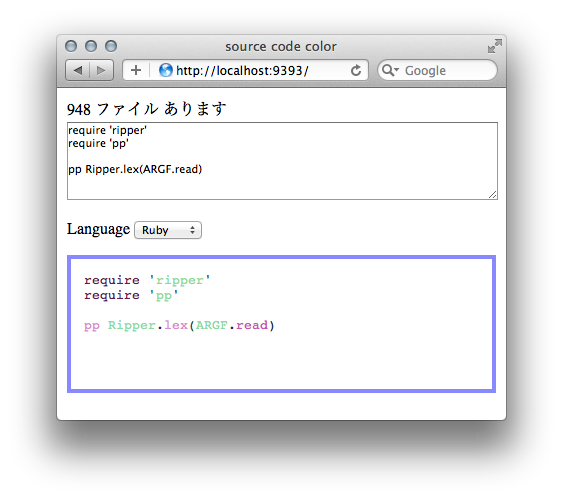
\includegraphics[scale=0.8]{editor-screenshot-example.png}
   \caption{字句解析に成功した場合のエディタのスクリーンショット}
   \label{editor-screenshot-example}
  \end{figure}

  \begin{figure}[htbp]
   \centering
   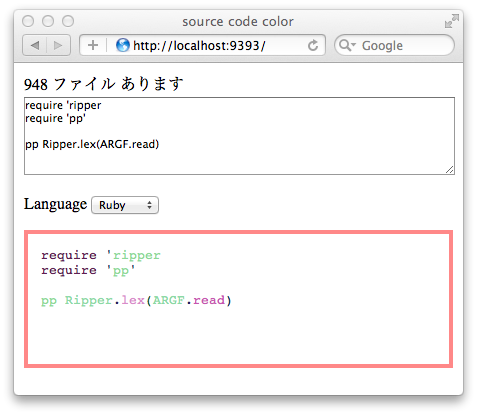
\includegraphics[scale=0.8]{editor-screenshot-example-fail.png}
   \caption{字句解析失敗した場合のエディタのスクリーンショット}
   \label{editor-screenshot-example-fail}
  \end{figure}

  \subsection{字句解析に成功する場合}
  ここでは,色の決定について,字句解析が成功する場合と失敗する場合のそれぞれについて,具体例を示す.

  前準備として,GitHubから,主にRubyで書かれて,ブックマークに登録した人の人数が多いリポジトリをクロールしている.クロールしたリポジトリのURLを付録A(全部で160箇所)に示す.

  以下のRubyのプログラムの色付けを,順に見ていく.

  \begin{framed}
\begin{verbatim}
require 'rubygems'
  \end{verbatim}
\end{framed}

  まず,クライアントからサーバーにHTTPリクエストが送られる.

\begin{framed}
\begin{verbatim}
data: require 'rubygems'
mime_type: application/ruby
\end{verbatim}
\end{framed}

サーバーは,リクエストを受け取ると,入力されたソースコードを,Rubyの字句解析器を使って字句解析する.
字句解析すると,以下のトークンの配列になる.
トークンは,トークンの値と,トークンのクラスを持っている.

\begin{framed}
\begin{verbatim}
[{:value=>"require", :class=>"on_ident"},
 {:value=>" ", :class=>"on_sp"},
 {:value=>"'", :class=>"on_tstring_beg"},
 {:value=>"rubygems", :class=>"on_tstring_content"},
 {:value=>"'", :class=>"on_tstring_end"}]
\end{verbatim}
\end{framed}

各トークンの出現回数をデータベースに問い合わせる.
以下の結果が得られたとする.
\begin{framed}
\begin{verbatim}
{"require"=>465, "'"=>644, "rubygems"=>25}
\end{verbatim}
\end{framed}

次に,全部でいくつのファイルがデータベースに登録されているかを問い合わせる.
この場合は1029であったとする.
すると,各トークンの出現確率は以下である.

\begin{itemize}
 \item require: 45パーセント
 \item ': 62パーセント
 \item rubygems: 2パーセント
\end{itemize}

輝度は以下の式で決める.

\begin{framed}
\begin{verbatim}
輝度(出現確率) = (0.6 - 出現確率) * 100
ただし,出現確率が0のときは70
ただし,輝度が0より小さいときは0
\end{verbatim}
\end{framed}

輝度は0から100で,0は真っ黒,100は真っ白である.

次に,色相を決める.
色相は,トークンのクラスの出現確率が大きいものが青っぽくなるように割り当てる.

トークンごとの出現回数から色相を決定する方法は以下の通りである.
\begin{itemize}
 \item 出現確率が大きいものから小さいものの順に割り当てていく.
 \item 出現確率が一番大きいクラスを180度(水色)に割り当てる.
 \item 以降のクラスは,出現確率に比例して隣のクラスから離した場所に割り当てる.
 \item 割り当ては,180度から0度に角度が下がっていく方向と,180度から360度に上がっていく方向の交互に割り当てる.
 \item 一番小さいものは0度(赤)に割り当てられる.
\end{itemize}

これにより,各トークンのクラスの色相は以下のように決定される.

\begin{framed}
\begin{verbatim}
{"on_words_beg"=>0,
 "on_embdoc_end"=>0,
 "on_embdoc_beg"=>0,
 "on_backtick"=>0,
 "on_sp"=>0,
 "on_CHAR"=>0,
 "on_embdoc"=>0,
 "on_cvar"=>0,
 "on_backref"=>0,
 "on_words_sep"=>0,
 "on_qwords_beg"=>0,
 "on_heredoc_end"=>0,
 "on_heredoc_beg"=>0,
 "on_gvar"=>0,
 "on_float"=>0,
 "on_semicolon"=>0,
 "on_regexp_beg"=>0,
 "on_regexp_end"=>359,
 "on_embexpr_beg"=>1,
 "on_lbrace"=>358,
 "on_int"=>4,
 "on_rbrace"=>354,
 "on_rbracket"=>9,
 "on_lbracket"=>348,
 "on_ivar"=>15,
 "on_symbeg"=>342,
 "on_const"=>25,
 "on_rparen"=>327,
 "on_lparen"=>41,
 "on_tstring_beg"=>312,
 "on_tstring_end"=>56,
 "on_tstring_content"=>296,
 "on_comma"=>73,
 "on_comment"=>279,
 "on_period"=>91,
 "on_op"=>258,
 "on_kw"=>117,
 "on_ident"=>225}
\end{verbatim}
\end{framed}

各トークンの色は以下のように決定する.

\begin{itemize}
 \item require: hsl(225, 50\%, 14\%)
 \item ': hsl(312, 50\%, 0\%)
 \item rubygems: hsl(296, 50\%, 57\%)
\end{itemize}

サーバーからの返されるレスポンスは以下である.JSON形式でシリアライズされている.

\begin{framed}
\begin{verbatim}
{"tokens"=>
  [{"value"=>"require",
    "count"=>465,
    "rate"=>0.4518950437317784,
    "token_class"=>"on_ident",
    "color"=>"hsl(225, 50%, 14%)"},
   {"value"=>" ",
    "count"=>0,
    "rate"=>0.0,
    "token_class"=>"on_sp",
    "color"=>"hsl(0, 50%, 60%)"},
   {"value"=>"'",
    "count"=>644,
    "rate"=>0.6258503401360545,
    "token_class"=>"on_tstring_beg",
    "color"=>"hsl(312, 50%, 0%)"},
   {"value"=>"rubygems",
    "count"=>25,
    "rate"=>0.024295432458697766,
    "token_class"=>"on_tstring_content",
    "color"=>"hsl(296, 50%, 57%)"},
   {"value"=>"'",
    "count"=>644,
    "rate"=>0.6258503401360545,
    "token_class"=>"on_tstring_end",
    "color"=>"hsl(56, 50%, 0%)"},
   {"value"=>"\n",
    "count"=>0,
    "rate"=>0.0,
    "token_class"=>"on_nl",
    "color"=>"hsl(0, 50%, 60%)"}],
 "is_valid"=>true}
\end{verbatim}
\end{framed}


エディタで色付けすると,図\ref{example-code-can-compile}のように色付けされる.

  \begin{figure}[htbp]
   \centering
   
\includegraphics[scale=0.8]{example-code-can-compile.png}
   \caption{動作例}
   \label{example-code-can-compile}
  \end{figure}


  以下のような手順で表示できる.

\begin{itemize}
 \item tokens にトークンのArrayであるので,順に見る
 \item valueがトークンの内容,colorが色であるので,valueをcolorの色で表示する
\end{itemize}

tokensのvalueを連結すると,色付けされた,もとのソースコードが復元される.

  図\ref{example-code-can-compile}の色付け結果を見ると,requireが頻出すること,rubygemsは多く出現するが,requireほどは多くないこと,rubygemsは青っぽいので,多く出現するクラスのトークンであること,がわかる.

  \subsection{字句解析に失敗する場合}

  前節では字句解析できる場合の実行を説明した.
  本節では字句解析できない場合について説明する.

  字句解析に成功したかどうかは,字句解析モジュールの返り値として得られるようになっている.
  字句解析に失敗した場合は,空白と正規表現でトークンを切り分ける.

  以下のプログラムを色付けすることを考える.

\begin{framed}
\begin{verbatim}
'require 'rubygems'
\end{verbatim}
\end{framed}

行頭に'が入っているため,このプログラムは字句解析に失敗する.
字句解析に失敗したときは適当な正規表現でソースコードをトークンに切り出すことを試みる.
以下の正規表現をセパレータとして分割する.
空白もしくは単語境界にマッチする.
単語境界とは,英数字と非英数字の間にマッチする.

\begin{framed}
\begin{verbatim}
/(\s+)|\b/
\end{verbatim}
\end{framed}

ソースコードを上の正規表現ごとに分割し,空白文字は取り除くと,以下のように分割される.

\begin{framed}
\begin{verbatim}
["'", "require", " ", "'", "rubygems", "'"]
\end{verbatim}
\end{framed}

次に,トークンのクラスを推測する.

本システムの字句解析器は,字句解析した際に,トークンのクラスが何であったかをデータベースに保存している.データベースから,各トークンを字句解析した際にどのクラスが何回出現したかを取得する.

それぞれ以下の通りである.

\begin{framed}
\begin{verbatim}
[{"count"=>977,
  "token_class"=>{"on_ident"=>977},
  "value"=>"require"},
 {"count"=>14350,
  "token_class"=>
   {"on_tstring_beg"=>7130,
    "on_tstring_content"=>69,
    "on_tstring_end"=>7145,
    "on_words_sep"=>6},
  "value"=>"'"},
 {"count"=>25,
  "token_class"=>{"on_tstring_content"=>25},
  "value"=>"rubygems"}]
\end{verbatim}
\end{framed}

出現回数の一番多いものを利用するので,各トークンのクラスは以下であると推測する.

\begin{itemize}
 \item ': on\_tstring\_beg
 \item require: on\_ident
 \item rubygems: on\_tstring\_content
\end{itemize}

ここで推測したクラスによって,色相を決定する.

正規表現で切り分けるのに失敗したトークンや,はじめて出現したトークンなど,データベースに対応するレコードが存在しない場合がある.
データベースに対応するレコードが存在しない場合は,未定義というクラスを割り当てる.
未定義のクラスは色相が0度で,輝度は60\%である.

サーバーは以下のJSONを返す.

\begin{framed}
\begin{verbatim}
{:tokens=>
  [{:value=>"'",
    :count=>644,
    :rate=>0.6258503401360545,
    :token_class=>"on_tstring_end",
    :color=>"hsl(56, 50%, 0%)"},
   {:value=>"require",
    :count=>465,
    :rate=>0.4518950437317784,
    :token_class=>"on_ident",
    :color=>"hsl(225, 50%, 14%)"},
   {:value=>" ",
    :count=>0,
    :rate=>0.0,
    :token_class=>"?",
    :color=>"hsl(0, 50%, 60%)"},
   {:value=>"'",
    :count=>644,
    :rate=>0.6258503401360545,
    :token_class=>"on_tstring_end",
    :color=>"hsl(56, 50%, 0%)"},
   {:value=>"rubygems",
    :count=>25,
    :rate=>0.024295432458697766,
    :token_class=>"on_tstring_content",
    :color=>"hsl(296, 50%, 57%)"},
   {:value=>"'",
    :count=>644,
    :rate=>0.6258503401360545,
    :token_class=>"on_tstring_end",
    :color=>"hsl(56, 50%, 0%)"}]}
\end{verbatim}
\end{framed}

色付け結果を図\ref{example-code-can-not-compile}に示す.
内部的には字句解析していないにも関わらず,字句解析して色付けした結果とほぼ同じ色がついている.

  \begin{figure}[htbp]
   \centering
   
\includegraphics[scale=0.8]{example-code-can-not-compile.png}
   \caption{字句解析に失敗した場合の動作例}
   \label{example-code-can-not-compile}
  \end{figure}

  \section{考察}
  ここでは,2つの観点から考察を述べる.

  \subsection{輝度の差による情報の提示}

  通常のシンタックスハイライトは,たとえば,識別子は緑,といったように,同じクラスのトークンは同じ色になる.
  本システムは,出現確率によって輝度を変更し,そのトークンがどの程度出現するものかを示す.
  本節では輝度の差による情報の提示について述べる.

  以下のソースコードを本システムで表示した例を図\ref{example-identifier-color}に示す.

\begin{framed}
\begin{verbatim}
list.each.inject.injectt
\end{verbatim}
\end{framed}

  \begin{figure}[htbp]
   \centering
   
\includegraphics[scale=0.8]{example-identifier-color.png}
   \caption{動作例}
   \label{example-identifier-color}
  \end{figure}

  メソッド名として書かれている,each,inject,injectt,について見る.
  色の明るさについて見ると,each,inject,injectt,という順に明るくなっている.
  このことから,世の中のソースコードでは,each $>$ inject $>$ injectt という順に出現していることがわかる.
  eachは,リストを順番に評価するメソッドで,injectはリストの畳み込み操作のメソッドである.
  畳み込み操作より,順に評価する機会のほうが多いため,injectよりeachの方が多く出現していることは納得できる.
  また,injecttは,たいへん明るい.
  Rubyの標準ライブラリにinjecttというメソッドは存在せず,このコードを実行すると,injecttを呼ぼうとして実行時エラーが出て終了する.
  この明るさは,出現確率が0のときの明るさである.
  世の中に存在しないトークンを書くことはあまりないため,何かの間違いである可能性がある.

  \subsection{正規表現によるシンタックスハイライトとの比較}
  正規表現を用いずに,従来手法と同じような色をつけることができた.
  従来手法では見ずらくなっていたコードも,見やすく色付けすることができた.
  従来手法では判別できなかった,トークンの出現確率を示すことができた.

  字句解析に失敗する場合,従来手法ではソースコード全体が変な色になっていたので,エラーがあることが心理的に分かりやすくなっていたが,本システムでは,ソースコード全体が変な色になるということは起きない.
  したがって,従来手法のように,ソースコード全体の色が変になっているときは,どこかのクオートを閉じ忘れている,といった推測をしにくくなる.

  字句解析に失敗したとき,空白もしくは単語境界で分割するので,一つのトークンに記号と英数字が混ざっていると,うまく分割できない.
  Perlでは,変数名の前に記号を書き,変数の型を示すので,Perlで,字句解析に失敗すると,変数名が正しく分割されず,よい結果を得られない.
  各言語に対して,字句解析と同様に,字句解析に失敗したときに用いる正規表現を記述できるようにすると,Perlのソースコードを分割するときには,先頭が記号で英数字が続く場合は一つのトークンと見なす,ということもできる.
  しかし,そうすると,従来手法と同じように,言語ごとに正規表現をメンテナンスすることになってしまう.

    % しかし,エラー箇所の提示は,シンタックスハイライトの機能ではなく,別に,コンパイルに失敗した箇所を示すプログラムを導入すれば分かることなので,そのようなツールと組み合わせて利用すれば,本システムは有効であると考えられる.

  これまでは正規表現のマッチだけで色付けできていたが,本システムでは,先に,統計用のソースコードをクロールしたり,色付け対象言語を字句解析するプログラムを用意し,システムに組込む必要がある.
  また,従来手法ではシンタックスハイライトプログラムはエディタ上で動作していたため,ユーザーが増えてもスケールしていたが,本システムでは,字句解析やデータベースへのアクセスなどをサーバーで行うため,ユーザーが増えると,負荷が集中し,色付けに時間がかかってしまうことなどが考えられる.
  これは,ユーザーが増えるに従ってサーバーを増やすことなどによって対処できると考えられる.


  \clearpage
 \section{おわりに}
 本論文ではソースコードの統計情報と,字句解析によって,シンタックスハイライトを行うシステムを提案した.
 本システムを利用することで,ソースコードが見やすくなり,プログラミング環境が良くなると思われる.

 今後の課題として,本システムをシンタックスハイライトサーバーとして動作させるテキストエディタの実装がある.
 EmacsやEclipseなどのエディタはプラグイン形式でコードを実行できるので,そのような仕組みを利用すれば実装できると思われる.
 また,ユーザーが増えてもスケールするような実装に変更することも課題である.

 \acknowledgement
 本論文の執筆において,有益なる御教授,御示唆をいただきました000大学0000学部0000教授に深く感謝の意を表します.

 また,その他さまざまな面で御助言をいただきました000館大学0000学部000000000000000000研究室の皆様に深く感謝の意を表します.

  \clearpage

  \begin{thebibliography}{9}
   \bibitem{bib:nano} GNU nano, http://www.nano-editor.org/,2012年2月6日
   \bibitem{bib:vim} welcome home : vim online, http://www.vim.org/
   \bibitem{bib:emacs} GNU Emacs - GNU Project - Free Software Foundation (FSF),http://www.gnu.org/software/emacs/,2012年2月6日
   \bibitem{bib:emacs-oreilly} Debra Cameron, James Elliott, Marc Loy, Eric Raymond, Bill Rosenblatt 著,半田 剣一,宮下 尚 監訳,新井 貴之,鈴木 和也 訳,入門 GNU Emacs 第3版,オライリー・ジャパン,2007
   \bibitem{bib:emacs-org} Org: Your Life in Plain Text,http://orgmode.org/,2012年2月8日
   \bibitem{bib:emacs-yatex} YaTex,http://www.math.s.chiba-u.ac.jp/matsu/emacs/emacs21/yatex.html,2012年2月8日
   \bibitem{bib:compiler} 中田育男,コンパイラ,産業図書,1981
  \end{thebibliography}

  \clearpage

\def\thesection{}
\setcounter{section}{0}
\section{付録A クロールしたリポジトリのURL}

% うまくいかなかったのでappendixとか使っていません

\begin{verbatim}
     1	git://github.com/aaronchi/jrails.git
     2	git://github.com/adamsalter/sitemap_generator.git
     3	git://github.com/adamwiggins/yaml_db.git
     4	git://github.com/adzap/validates_timeliness.git
     5	git://github.com/amatsuda/kaminari.git
     6	git://github.com/andi/simple-navigation.git
     7	git://github.com/andre/geokit-gem.git
     8	git://github.com/andre/geokit-rails.git
     9	git://github.com/apotonick/apotomo.git
    10	git://github.com/apotonick/cells.git
    11	git://github.com/appelier/bigtuna.git
    12	git://github.com/bcardarella/client_side_validations.git
    13	git://github.com/be9/acl9.git
    14	git://github.com/berk/tr8n.git
    15	git://github.com/binarylogic/authlogic_example.git
    16	git://github.com/binarylogic/memorylogic.git
    17	git://github.com/brendanlim/mobile-fu.git
    18	git://github.com/browsermedia/browsercms.git
    19	git://github.com/bsag/tracks-old.git
    20	git://github.com/chiliproject/chiliproject.git
    21	git://github.com/chrislloyd/gravtastic.git
    22	git://github.com/cloudhead/more.git
    23	git://github.com/codebrew/backbone-rails.git
    24	git://github.com/courtenay/altered_beast.git
    25	git://github.com/crafterm/sprinkle.git
    26	git://github.com/crowdint/rails3-jquery-autocomplete.git
    27	git://github.com/cucumber/cucumber-rails.git
    28	git://github.com/darthapo/comatose.git
    29	git://github.com/dbloete/masquerade.git
    30	git://github.com/dchelimsky/rspec-rails.git
    31	git://github.com/dcrec1/inploy.git
    32	git://github.com/dejan/auto_html.git
    33	git://github.com/dhh/tolk.git
    34	git://github.com/diaspora/diaspora.git
    35	git://github.com/dnclabs/client_side_validations.git
    36	git://github.com/DocSavage/rails-authorization-plugin.git
    37	git://github.com/documentcloud/jammit.git
    38	git://github.com/drhenner/ror_ecommerce.git
    39	git://github.com/drnic/ruby-on-rails-tmbundle.git
    40	git://github.com/dsboulder/query_reviewer.git
    41	git://github.com/edavis10/redmine.git
    42	git://github.com/eladmeidar/rails_indexes.git
    43	git://github.com/elevation/event_calendar.git
    44	git://github.com/engineyard/rails_metrics.git
    45	git://github.com/fabrik42/acts_as_api.git
    46	git://github.com/fatfreecrm/fat_free_crm.git
    47	git://github.com/fdv/typo.git
    48	git://github.com/ffmike/BigOldRailsTemplate.git
    49	git://github.com/Fingertips/passengerpane.git
    50	git://github.com/flyerhzm/bullet.git
    51	git://github.com/flyerhzm/rails_best_practices.git
    52	git://github.com/fortuity/rails3-mongoid-devise.git
    53	git://github.com/fortuity/rails3-subdomain-devise.git
    54	git://github.com/freelancing-god/thinking-sphinx.git
    55	git://github.com/fudgestudios/bort.git
    56	git://github.com/gnufied/backgroundrb.git
    57	git://github.com/gregbell/active_admin.git
    58	git://github.com/grempe/amazon-ec2.git
    59	git://github.com/grimen/validatious-on-rails.git
    60	git://github.com/grosser/parallel_tests.git
    61	git://github.com/hcatlin/make_resourceful.git
    62	git://github.com/igrigorik/async-rails.git
    63	git://github.com/indirect/haml-rails.git
    64	git://github.com/indirect/rails3-generators.git
    65	git://github.com/insoshi/insoshi.git
    66	git://github.com/jamesgolick/resource_controller.git
    67	git://github.com/jcasimir/draper.git
    68	git://github.com/jejacks0n/navigasmic.git
    69	git://github.com/jim/carmen.git
    70	git://github.com/jlecour/geokit-rails3.git
    71	git://github.com/jm/rails-templates.git
    72	git://github.com/jnicklas/carrierwave.git
    73	git://github.com/jnunemaker/crack.git
    74	git://github.com/josevalim/enginex.git
    75	git://github.com/josevalim/rails-footnotes.git
    76	git://github.com/joshfrench/rakismet.git
    77	git://github.com/joshmh/globalize2.git
    78	git://github.com/justinfrench/formtastic.git
    79	git://github.com/jviney/acts_as_taggable_on_steroids.git
    80	git://github.com/kete/tiny_mce.git
    81	git://github.com/kfaustino/rails-templater.git
    82	git://github.com/kristianmandrup/cream.git
    83	git://github.com/langalex/culerity.git
    84	git://github.com/lazyatom/engines.git
    85	git://github.com/leppert/remotipart.git
    86	git://github.com/lucasefe/themes_for_rails.git
    87	git://github.com/maccman/acts_as_recommendable.git
    88	git://github.com/maccman/saasy.git
    89	git://github.com/markbates/coffeebeans.git
    90	git://github.com/markevans/dragonfly.git
    91	git://github.com/mbleigh/acts-as-taggable-on.git
    92	git://github.com/mbleigh/seed-fu.git
    93	git://github.com/mbleigh/subdomain-fu.git
    94	git://github.com/mbleigh/twitter-auth.git
    95	git://github.com/michelson/lazy_high_charts.git
    96	git://github.com/mileszs/wicked_pdf.git
    97	git://github.com/mintdigital/asset_hat.git
    98	git://github.com/mislav/will_paginate.git
    99	git://github.com/mmangino/facebooker.git
   100	git://github.com/mxcl/homebrew.git
   101	git://github.com/mynewsdesk/translate.git
   102	git://github.com/NoamB/sorcery.git
   103	git://github.com/NUBIC/surveyor.git
   104	git://github.com/NZKoz/rails_xss.git
   105	git://github.com/p8/table_builder.git
   106	git://github.com/paneq/active_reload.git
   107	git://github.com/paolodona/rails-widgets.git
   108	git://github.com/pauldowman/ec2onrails.git
   109	git://github.com/pelle/oauth-plugin.git
   110	git://github.com/pivotal/desert.git
   111	git://github.com/plataformatec/devise.git
   112	git://github.com/plataformatec/mail_form.git
   113	git://github.com/plataformatec/responders.git
   114	git://github.com/plataformatec/simple_form.git
   115	git://github.com/prior/prawnto.git
   116	git://github.com/pullmonkey/open_flash_chart.git
   117	git://github.com/purzelrakete/workling.git
   118	git://github.com/quickleft/prologue.git
   119	git://github.com/radar/forem.git
   120	git://github.com/radar/rboard.git
   121	git://github.com/rails/pjax_rails.git
   122	git://github.com/rails/rails.git
   123	git://github.com/rails-sqlserver/activerecord-sqlserver-adapter.git
   124	git://github.com/railsmachine/moonshine.git
   125	git://github.com/railstutorial/sample_app.git
   126	git://github.com/raul/translate_routes.git
   127	git://github.com/resolve/refinerycms.git
   128	git://github.com/rspec/rspec-rails.git
   129	git://github.com/ryanb/cancan.git
   130	git://github.com/ryanb/complex-form-examples.git
   131	git://github.com/ryanb/nested_form.git
   132	git://github.com/ryanb/nifty-generators.git
   133	git://github.com/sbecker/asset_packager.git
   134	git://github.com/spree/spree.git
   135	git://github.com/Squeegy/fleximage.git
   136	git://github.com/stevenbristol/lovd-by-less.git
   137	git://github.com/stffn/declarative_authorization.git
   138	git://github.com/stonean/lockdown.git
   139	git://github.com/Sutto/barista.git
   140	git://github.com/svenfuchs/rails-i18n.git
   141	git://github.com/svenfuchs/routing-filter.git
   142	git://github.com/tablatom/hobo.git
   143	git://github.com/technoweenie/restful-authentication.git
   144	git://github.com/thetron/css3buttons_rails_helpers.git
   145	git://github.com/thoughtbot/clearance.git
   146	git://github.com/thoughtbot/factory_girl_rails.git
   147	git://github.com/thoughtbot/high_voltage.git
   148	git://github.com/thumblemonks/smurf.git
   149	git://github.com/tra/spawn.git
   150	git://github.com/trevorturk/eldorado.git
   151	git://github.com/twg/comfortable-mexican-sofa.git
   152	git://github.com/typus/typus.git
   153	git://github.com/wayneeseguin/dynamic_reports.git
   154	git://github.com/wr0ngway/rubber.git
   155	git://github.com/wvanbergen/request-log-analyzer.git
   156	git://github.com/wycats/rack-offline.git
   157	git://github.com/xaviershay/enki.git
   158	git://github.com/yaroslav/russian.git
   159	git://github.com/zapnap/resque_mailer.git
   160	git://github.com/zdennis/activerecord-import.git
\end{verbatim}


\end{document}
